\documentclass[xcolor=svgnames,handout]{beamer}
\usepackage[utf8]{inputenc}
\usepackage[english]{babel}

\usetheme{Sybila} 

\title[Noi ai tempi dei social network e del cloud computing]{La privacy ai tempi di Internet \\ tra social network e cloud computing}
\author{Fabrizio Soppelsa \\ fsoppelsa@oltrelinux.com}
\date{}

\begin{document}
% --------------------------- SLIDE --------------------------------------------
\frame[plain]{\titlepage}
% ------------------------------------------------------------------------------
% --------------------------- SLIDE --------------------------------------------
\begin{frame}
	\frametitle{Di cosa vi parlerò}

	\begin{enumerate}
				\pause
		\item Privacy: un rischio concreto?
				\pause
		\item Modello chiuso vs. modello aperto
				\pause
		\item Le trasmissioni dati su Internet
				\pause
		\item Le vostre informazioni in giro per il mondo
				\pause
		\item Il cloud che tutti amano è comodo, ma?
				\pause
		\item Soluzioni ed idee per contromisure
	\end{enumerate}
\end{frame}
% ------------------------------------------------------------------------------
\begin{frame}
	\frametitle{Privacy}

	\begin{block}{
\includegraphics[width=16px]{img/dictionary.png}}
		{\bf Diritto} alla riservatezza delle informazioni personali e della propria vita privata.
	\end{block}

		\pause

	\visible<2->{
	\begin{block}{
\includegraphics[width=16px]{img/warranty.png}}
		 ``Sovranità su di sé''
	\end{block}
	}
		
		\pause

	\visible<3->{
	\begin{block}{
\includegraphics[width=16px]{img/danger.png}}
		 Internet non è stata concepita per scambiare o gestire dati sensibili.
	\end{block}
	}

\end{frame}

\begin{frame}
	\frametitle{Reati contro la privacy}

	\begin{itemize}
			\item Violazione, sottrazione e soppressione di comunicazioni.
			\item Falsificazione, alterazione e diffusione di comunicazioni.
			\item Uso di apparecchiature per le intercettazioni.
			\item Rivelazione del contenuto di documenti segreti.
			\item Accesso non autorizzato ad un sito.
			\item Spionaggio.
	\end{itemize}

		\pause

	\visible<2->{
			\begin{block}{
\includegraphics[width=16px]{img/important.png}}
				Come vengono usate le informazioni che {\bf NOI} diamo.
			\end{block}
	}
\end{frame}

\def\imagetop#1{\vtop{\null\hbox{#1}}}

\begin{frame}
	\frametitle{Il software locale}

	\begin{block}{Trattamento dei dati}
		\begin{center}
		\begin{tabular}{ c c }
				\imagetop{
\includegraphics[height=74px,raise=-\height]{img/closed.png}} & \imagetop{
\includegraphics[height=80px,raise=-\height]{img/open.png}} \\\hline
				  \pause
				  Scatola chiusa & \pause Scatola aperta \\
				  \pause
				  Procedure segrete & \pause Procedure note \\
				  \pause
				  Spyware? & \pause Niente segreti \\
		\end{tabular}
		\end{center}
	\end{block}
\end{frame}

\begin{frame}
	\frametitle{www.example.com}

	\begin{block}{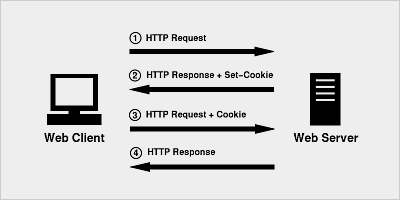
\includegraphics[width=150px]{img/request-response.png}}
			\begin{itemize}
						\pause
					\item Connessione al sito
						\pause
					\item Il server registra le attività
						\pause
					\item Uso dei {\bf cookie}
						\pause
					\item Rischio per la privacy?
			\end{itemize}
	\end{block}
\end{frame}

\begin{frame}
	\frametitle{Cookie}

	\begin{block}{
\includegraphics[width=70px]{img/cookie.jpg}}
			\begin{itemize}
						\pause
					\item Raccolta info su abitudini degli utenti
						\pause
					\item Salvataggio impostazioni
						\pause
					\item Pubblicità mirate
						\pause
					\item Abusi
						\pause
					\item Confine labile: non sempre possibile rifiutarli
			\end{itemize}
	\end{block}
\end{frame}

\begin{frame}
	\frametitle{Trasmissione password}

	\begin{block}{
\includegraphics[width=40px]{img/login.png}}
			\begin{itemize}
					\item Servizi: www, email, login remoti
						\pause
					\item Fidarsi solo di protocolli sicuri
						\pause
					\item \texttt{http{\bf s}}, \texttt{imap{\bf s}}, \texttt{{\bf s}sh}
						\pause
					\item Crittografia!
						\pause
					\item E solite raccomandazioni della nonna.
			\end{itemize}
	\end{block}
\end{frame}

\begin{frame}
	\frametitle{Email cifrate}

	\begin{block}{
\includegraphics[width=40px]{img/crypto.png}}
			\begin{itemize}
					\item Firma digitale
						\pause
					\item Cifratura dell'email
						\pause
					\item Crittografia a chiave pubblica
						\pause
					\item \texttt{gnupg}, keyserver noti e per esempio Enigmail
			\end{itemize}
	\end{block}
						
	\pause

	\visible<5->{
			\begin{center}
				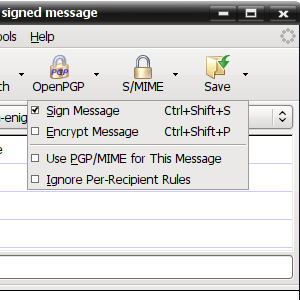
\includegraphics[width=100px]{img/pgp.png}
			\end{center}
	}
\end{frame}

\begin{frame}
	\frametitle{Routing anonimo}

	\begin{figure}[+ht]
			\begin{center}
					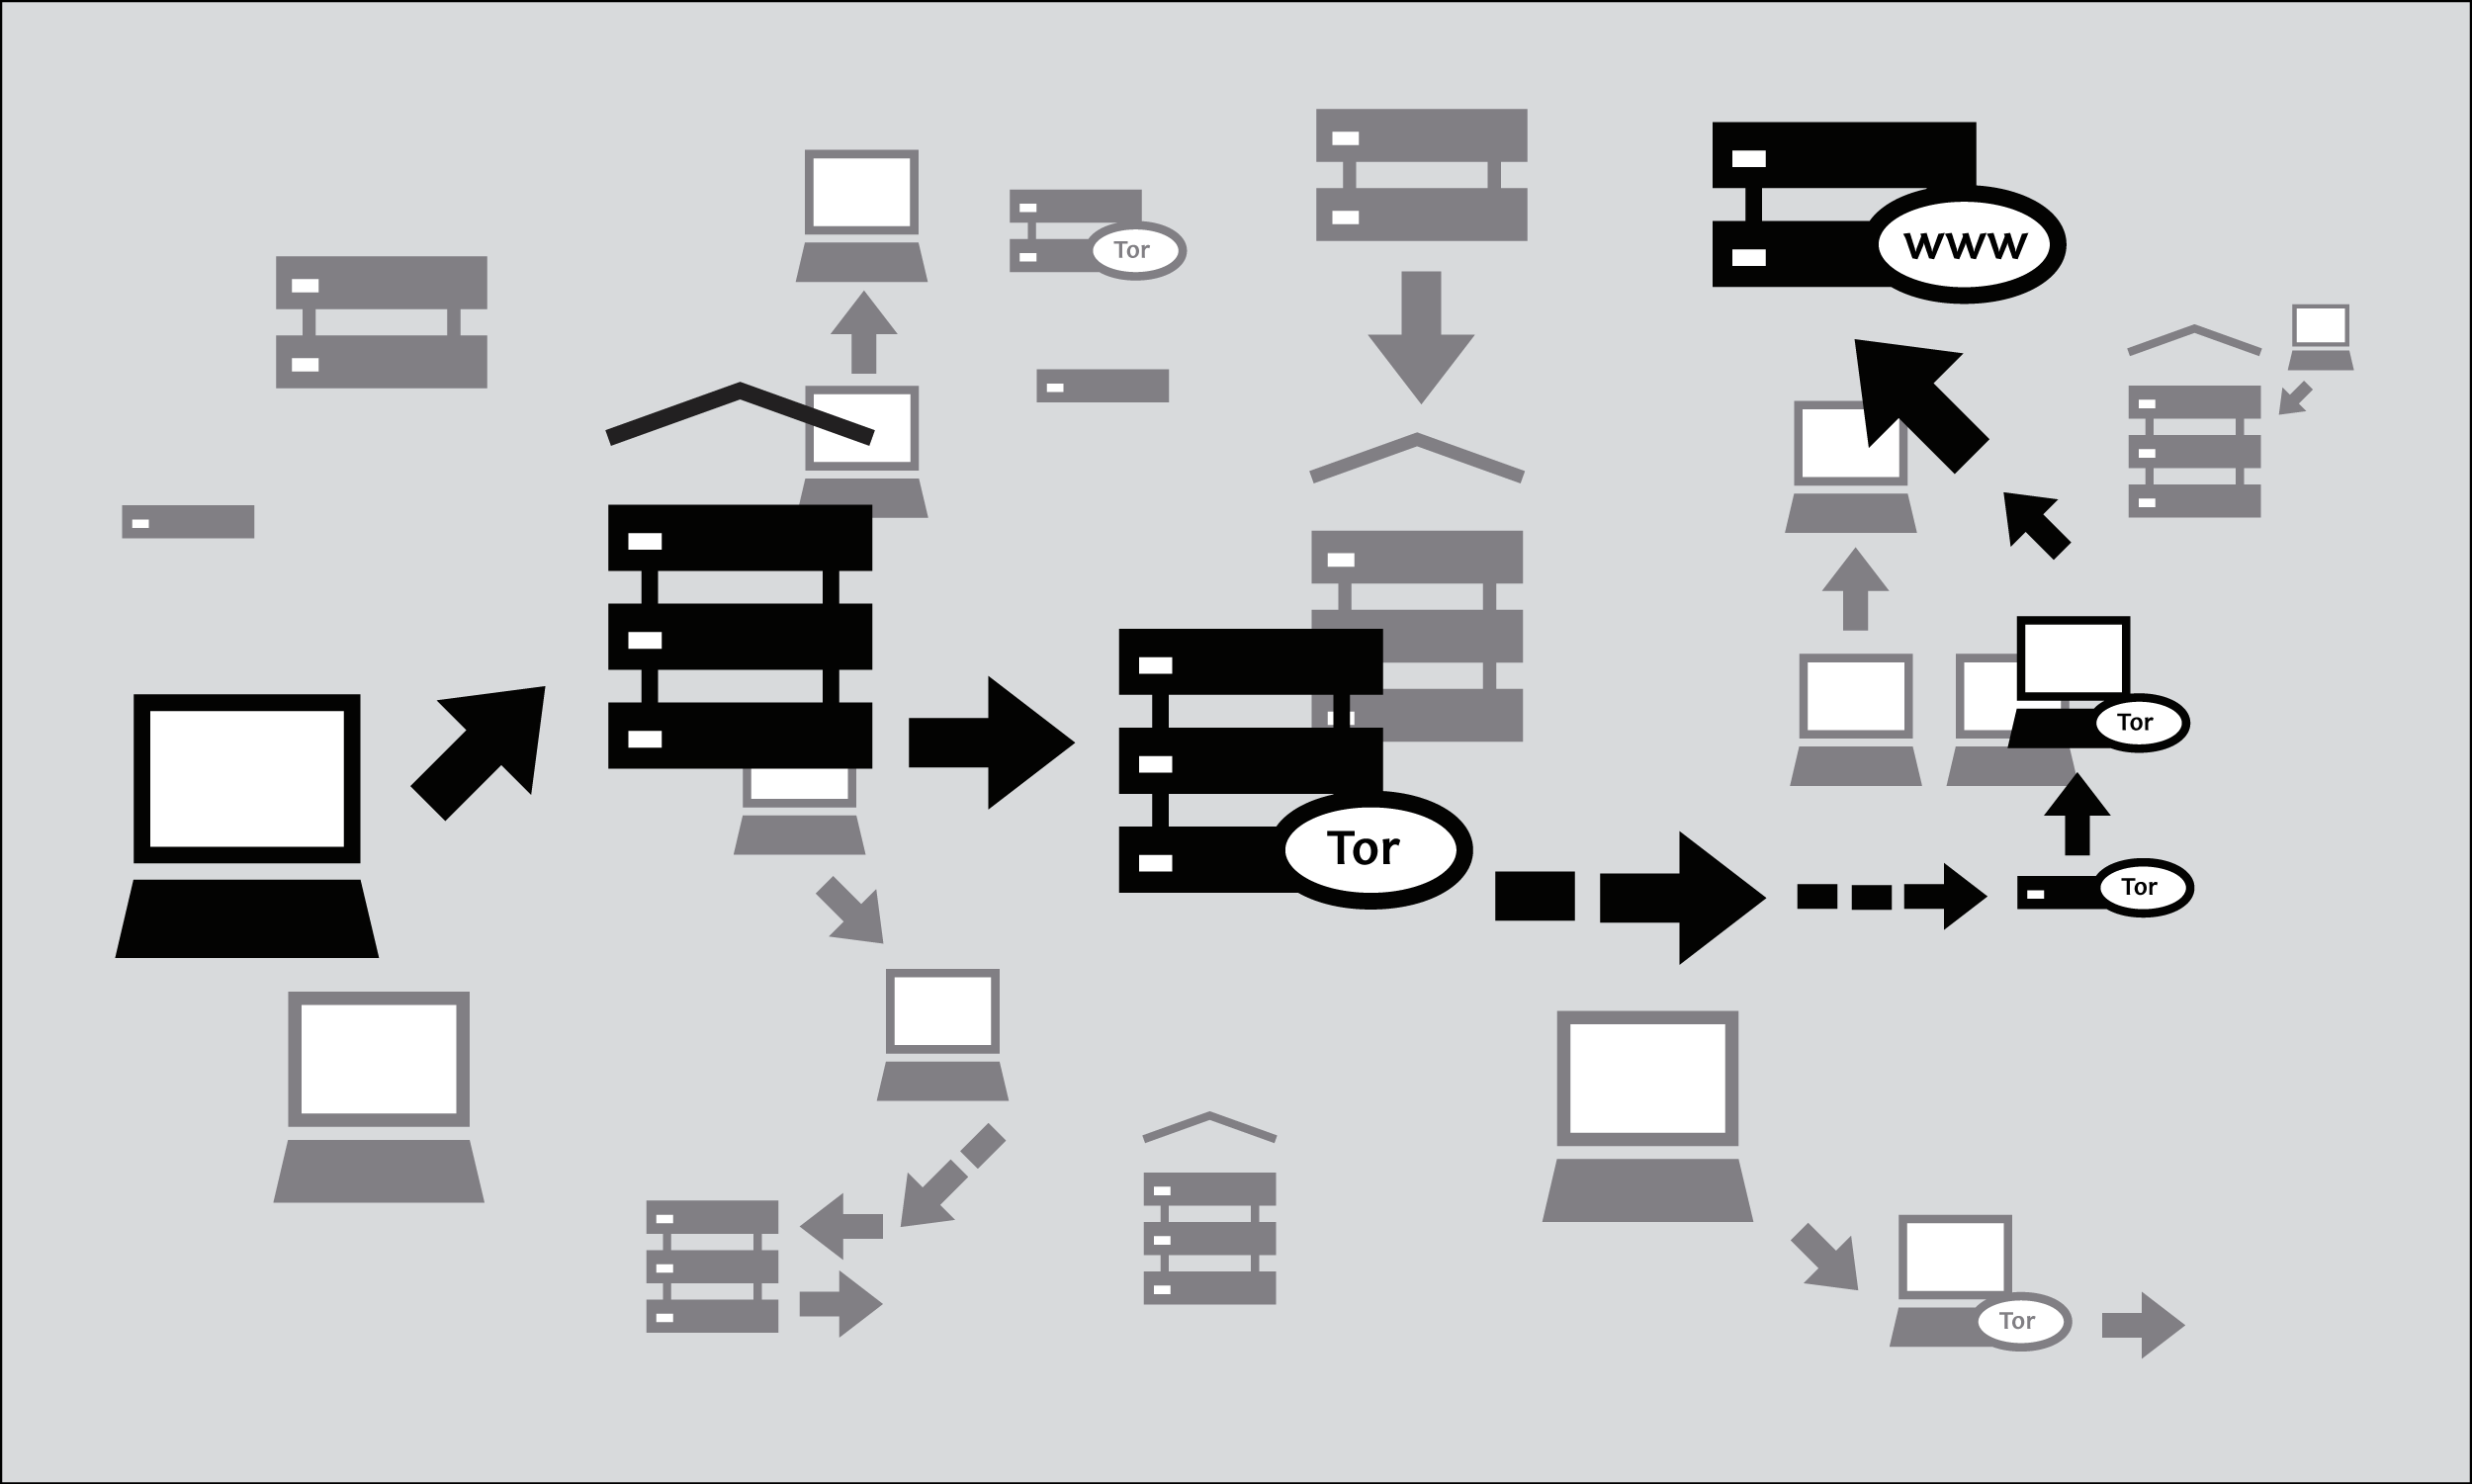
\includegraphics[width=280px]{img/tor.png}
			\end{center}
	\end{figure}

\end{frame}

\begin{frame}
	\frametitle{\texttt{http://tor.eff.org}}

	\begin{block}{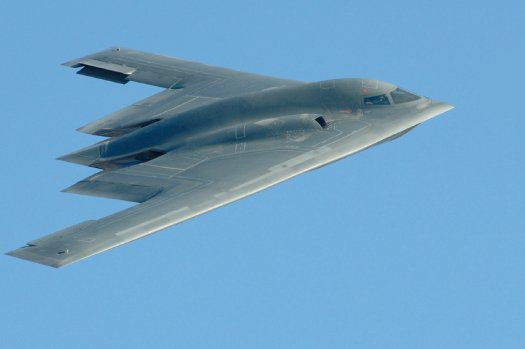
\includegraphics[width=40px]{img/stealth.jpg}}
			\begin{itemize}
					\item The Onion Router
						\pause
					\item Circuito virtuale casuale
						\pause
					\item Pacchetti incapsulati in n livelli crittografici
						\pause
					\item \texttt{yum install tor provoxy} \\
						  \texttt{apt-get install tor privoxy}
						\pause
					\item Sul browser impostare \texttt{localhost} come proxy server
			\end{itemize}
	\end{block}
						
	\visible<6->{
			\begin{center}
				
\includegraphics[width=100px]{img/tor_sticker.png}
			\end{center}
	}
\end{frame}

\begin{frame}
	\frametitle{Chi ha fame dei tuoi dati}

	\begin{figure}[+ht]
			\begin{center}
					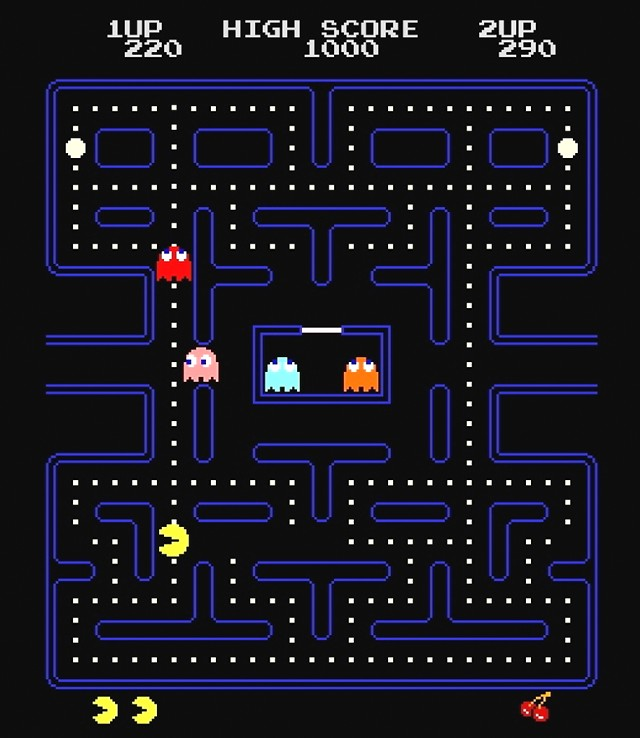
\includegraphics{img/pacman.jpg}
			\end{center}
	\end{figure}
\end{frame}

\begin{frame}
	\frametitle{Privacy sui social network}

	\begin{block}{
\includegraphics[width=40px]{img/social.png} \\ I rischi dei social network}
			\begin{enumerate}
						\pause
					\item Rischi relativi alla riservatezza dei dati
						\pause
					\item Rischi concernenti le identità digitali
						\pause
					\item Rischi di natura tecnologica
						\pause
					\item Rischi di natura sociale
			\end{enumerate}
	\end{block}
\end{frame}

\begin{frame}
	\frametitle{Privacy sui social network}

	\begin{block}{
\includegraphics[width=40px]{img/social.png} \\ I rischi dei social network}
			\begin{enumerate}
					\item {\bf Rischi relativi alla riservatezza dei dati}
					\item Rischi concernenti le identità digitali
					\item Rischi di natura tecnologica
					\item Rischi di natura sociale
			\end{enumerate}
	\end{block}
\end{frame}

\begin{frame}
	\frametitle{Scarsa trasparenza}

	\begin{block}{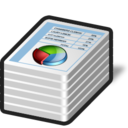
\includegraphics[width=40px]{img/data.png}}
			\begin{enumerate}
					\item Creazione dossier digitali
						\pause
					\item Dati e metadati associati (tag)
						\pause
					\item Quali garanzie?
						\pause
					\item Problemi nella cancellazione dei contenuti (solo disattivazione)
			\end{enumerate}
	\end{block}
\end{frame}

\begin{frame}
	\frametitle{Privacy sui social network}

	\begin{block}{
\includegraphics[width=40px]{img/social.png} \\ I rischi dei social network}
			\begin{enumerate}
					\item Rischi relativi alla riservatezza dei dati
					\item Rischi concernenti le identità digitali
					\item Rischi di natura tecnologica
					\item {\bf Rischi di natura sociale}
			\end{enumerate}
	\end{block}
\end{frame}

\begin{frame}
	\frametitle{Problematiche legate alla vita reale}

	\begin{block}{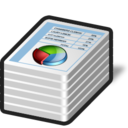
\includegraphics[width=40px]{img/data.png}}
			\begin{enumerate}
					\item Stalking
						\pause
					\item Cyberbullismo
						\pause
					\item Ricostruzione dati (es. codice fiscale)
						\pause
					\item Furto di identità
						\pause
					\item Risvolti sull'impiego
						\pause
					\item Predazione sessuale
			\end{enumerate}
	\end{block}
\end{frame}

\begin{frame}
	\frametitle{Un diamante è per sempre e anche\ldots}

	\begin{block}{
\includegraphics[width=30px]{img/warning.png}}
			\begin{enumerate}
					\item Quando inserisci i tuoi dati su un sito di social network, ne perdi il controllo
						\pause
					\item Il social network ha la licenza di usare i tuoi dati secondo i termini (anche per sempre)
						\pause
					\item La maggior parte dei siti di social network è all'estero sotto legislazioni straniere
						\pause
					\item Questi social network vivono grazie alle pubblicità mirate
						\pause
					\item Il loro business sei {\bf TU}
			\end{enumerate}
	\end{block}
\end{frame}


\begin{frame}
		\frametitle{Contromisure}

	\begin{block}{
\includegraphics[width=40px]{img/shield.png}}
			\begin{enumerate}
					\item Consapevolezza ed educazione
						\pause
					\item Password diverse
						\pause
					\item I dati sono quelli che inserisci {\bf TU}
						\pause
					\item Leggere i termini di contratto
						\pause
					\item Impostazioni visibilità
						\pause
					\item Rispettare la privacy degli altri
						\pause
					\item Segnalazione al Garante per la Privacy
			\end{enumerate}
	\end{block}
\end{frame}

\begin{frame}
	\frametitle{Il cloud computing (est. 1960)}

	\begin{center}
		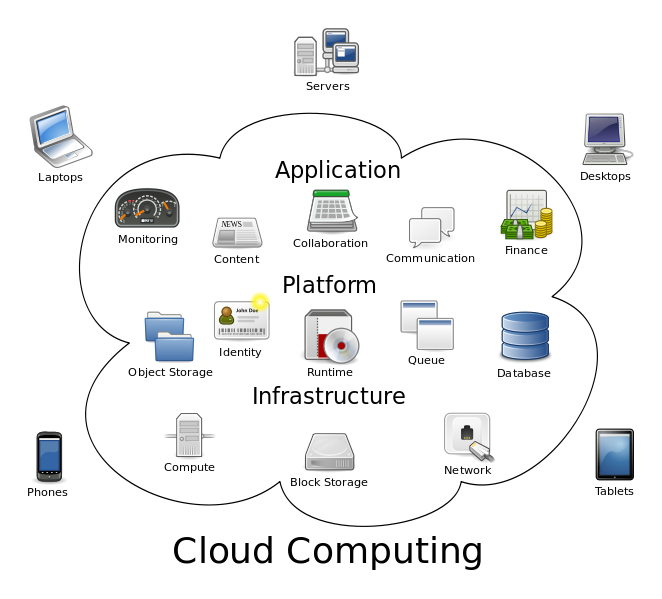
\includegraphics[width=200px]{img/cloud1.png}
	\end{center}
\end{frame}

\begin{frame}
	\frametitle{Che CaaSino}

	\begin{center}
		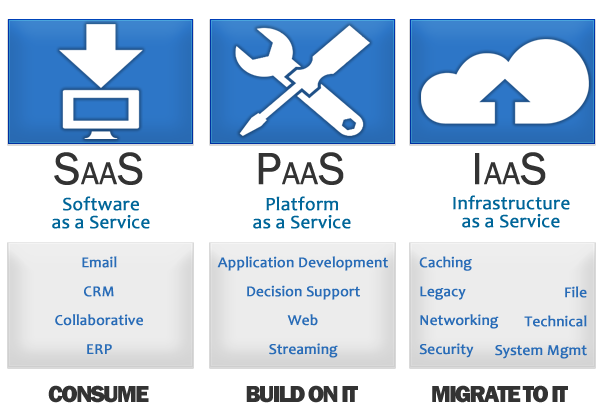
\includegraphics[width=200px]{img/service.png}
	\end{center}
\end{frame}

\begin{frame}
	\frametitle{Archiviazione nel cloud}

	\begin{block}{
\includegraphics[width=30px]{img/storage.png}}
			\begin{enumerate}
					\item Elaborazione, {\bf archiviazione}, recupero dati remoti
						\pause
					\item Risorse hardware e software distribuite
						\pause
					\item Comodo è comodo
						\pause
					\item Rende obsolete tecnologie obsolete
						\pause
					\item Costringe all'ordine
						\pause
					\item Architettura a server reali (ovviamente)
						\pause
					\item Amazon AWS, MobileMe, Azure, Dropbox, GitHub
			\end{enumerate}
	\end{block}
\end{frame}

\begin{frame}
	\frametitle{Punti di domanda}

	\begin{block}{
\includegraphics[width=30px]{img/cloud.png}}
			\begin{enumerate}
					\item Memorizzazione di dati sensibili?
						\pause
					\item Tutela della legislazione di quale paese?
						\pause
					\item Spionaggio industriale?
						\pause
					\item Accesso wireless e dalla rete cellulare?
						\pause
					\item Continuità del servizio?
						\pause
					\item Migrazione dei dati?
						\pause
					\item Furto d'identità
			\end{enumerate}
	\end{block}
\end{frame}

\begin{frame}
	\frametitle{Contromisure ed idee}

	\begin{block}{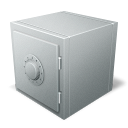
\includegraphics[width=20px]{img/safe.png}}
			\begin{enumerate}
					\item Avere idea di quello che si sta usando
						\pause
					\item Uso di protocolli aperti e della crittografia
						\pause
					\item Metodi di autenticazione seri, come {\bf OAuth}
						\pause
					\item Usare GeoIP
						\pause
					\item {\bf Costruirsi il proprio cloud}
						\pause
						\begin{itemize}
							\item ownCloud
								\pause
							\item OpenStack
								\pause
							\item Eucalyptus
								\pause
							\item OpenShift
						\end{itemize}
			\end{enumerate}
	\end{block}
\end{frame}

\begin{frame}
	\frametitle{Licenza}

	\begin{block}{Licenza MIT}
		\begin{itemize}
			\item Contenuto
			\item \LaTeX
			\item \texttt{Makefile}
			\item Icone
		\end{itemize}
	\end{block}

	\begin{center}
		{\bf \texttt{git clone git://github.com/fsoppelsa/ld2012.git}}
	\end{center}
\end{frame}

\begin{frame}
	\frametitle{C'est fini. Riflessioni?}

	\begin{center}
		
\includegraphics[width=150px]{img/q.jpg}
	\end{center}
\end{frame}
\end{document}
